\documentclass{article}

\usepackage{amsmath,amssymb,amsthm,mathtools,mathrsfs}
\usepackage[margin=1in]{geometry}
\usepackage{tikz}

\usetikzlibrary{arrows,automata}

\newtheorem{thm}{Theorem}
\newtheorem{lem}{Lemma}
\newtheorem{defin}{Definition}
\newtheorem*{cor}{Corollary}

\newenvironment{subproof}{%
  \begin{proof}[Subproof]%
}{%
  \end{proof}%
}

\title{Proof Golf in Axiom Systems}

\author{
Olive, Eamon \\
\texttt{olivee3@rpi.edu}
\and
Crisci, Michael \\
\texttt{criscm2@rpi.edu}
}

\begin{document}
\maketitle

\section{Introduction}

Proof Golf is an activity in which one chooses a logical truth and attempts to construct a proof of minimal ``size".
There are a two main ways that can be used to measure size.
The first is to count the number of symbols in the proof, this of course depends not only on the system in which your proof resides but a formal grammar for writing proof.
Then second is to count the number of steps in the proof, this depends pretty much only on the system in which you are constructing the proof since unlike symbols they tend to not depend on how you write the proof.
Between these two methods one may also choose to allow or disallow lematta.
Of course doing so requires us to decide how to score lematta.

For the sake of this paper we will consider the size of a proof to be the number of steps used, disallowing the use of lematta.
We will do this because it minimizes the number of arbitrary assumptions and in that way becomes more widely applicable similar problems.
We will also choose to work within the framework of a Hilbert Axiom system, in particular we will concern ourselves with the \L ukasiewicz system however our results are quite general.


\section{Basic Definitions and Results}

First let us lay out some definitions.
Some of these should probably be pretty familiar but others may be rather new.
The intention is to build a framework that will aid us in finding very short proofs,
once we define the relevant systems.

\begin{defin}
We shall define $\mathcal{A}$ to be a infinitely large set.
We will call its members \textbf{Atoms}.
\end{defin}

\begin{defin}
We shall define $\mathcal{V}$ to be a infinitely large set disjoint from the set of atoms.
We will call its members \textbf{Free Variables}.
\end{defin}

We won't talk about the internal structure of atoms and free variables, we only insist that the two are disjoint.
Now in practice there are no limitations on the number of atoms and free variables available but for convenience we will take atoms to be any capital Latin letter and free variables to be any lower case Greek letter.

\begin{defin}
A \textbf{well formed formula} will be defined as follows:
\begin{enumerate}
\item Every atom is a well formed formula.
\item If $\Phi$ is a well formed formula $\neg\Phi$ is also a well formed formula.
\item If both $\Phi$ and $\Psi$ are well formed formulae then $(\Phi\rightarrow\Psi)$ is a well formed formula.
\item No other statements are well formed formulae.
\end{enumerate}
We will call the set of all well formed formulae $\mathcal{W}$.
\end{defin}


\begin{defin}
A \textbf{formula} will be defined as follows:
\begin{enumerate}
\item Every atom is a formula.
\item Every free variable is a formula.
\item If $\Phi$ is a formula $\neg\Phi$ is also a formula.
\item If both $\Phi$ and $\Psi$ are formulae then $(\Phi\rightarrow\Psi)$ is a formula.
\item No other statements are formulae.
\end{enumerate}
We will call the set of all formulae $\mathcal{F}$.
\end{defin}

When talking about arbitrary formulae we will use capital Greek letters to stand in for complex statements.
For example if we wanted to talk about statements with $\rightarrow$ at the top level we would use the notation $\Phi \rightarrow \Psi$.
This is usually what free variables are used for but because free variables are objects we are concerned with we need to operate at the meta level.
This is purely notational.

\begin{defin}
Two formulae are \textbf{equal} if they are both generated by the same path in the grammar.
\begin{align*}
(\Phi \rightarrow \Psi) = (\Omega \rightarrow \Sigma) &\iff (\Phi = \Omega) \land (\Psi = \Sigma) \\
\neg \Phi = \neg \Psi &\iff \Phi = \Psi
\end{align*}
Formulae comprised solely of an atom or variable inherit equality from the atom or variable they are comprised of.
\end{defin}

\begin{defin}
The \textbf{set of free variables appearing in} a formula $\Phi$ will be denoted as $\Phi^\mathcal{V}$.
\setlength{\tabcolsep}{1pt}
\begin{center}
	\begin{tabular}{rclc}
		                               & $(\Phi \rightarrow \Psi)^\mathcal{V}$ & $=$ & $ \Phi^\mathcal{V} \cup \Psi^\mathcal{V}$ \\
		                               & $(\neg \Phi)^\mathcal{V}            $ & $=$ & $ \Phi^\mathcal{V}               $ \\
		$\Phi \in \mathcal{A} \implies$ & $\Phi^\mathcal{V}                   $ & $=$ & $ \{\}                    $ \\
		$\Phi \in \mathcal{V} \implies$ & $\Phi^\mathcal{V}                   $ & $=$ & $ \{\Phi\}                $
	\end{tabular}
\end{center}
\end{defin}

\begin{defin}
The \textbf{set of atoms appearing in} a formula $\Phi$ will be denoted as $\Phi^\mathcal{A}$.
\setlength{\tabcolsep}{1pt}
\begin{center}
	\begin{tabular}{rclc}
		                               & $(\Phi \rightarrow \Psi)^\mathcal{A}$ & $=$ & $ \Phi^\mathcal{A} \cup \Psi^\mathcal{A}$ \\
		                               & $(\neg \Phi)^\mathcal{A}            $ & $=$ & $ \Phi^\mathcal{A}               $ \\
		$\Phi \in \mathcal{V} \implies$ & $\Phi^\mathcal{A}                   $ & $=$ & $ \{\}                    $ \\
		$\Phi \in \mathcal{A} \implies$ & $\Phi^\mathcal{A}                   $ & $=$ & $ \{\Phi\}                $
	\end{tabular}
\end{center}
\end{defin}
\begin{defin}
The function $f : A \mapsto B$ \textbf{constrained to} a set $C \subseteq A$, denoted $f \mid A$ is a new function mapping
members of $C$ to members of $B$ such that:

\begin{align*}
\forall x \in C : (f \mid C) (x) = f (x)
\end{align*}
\end{defin}

\begin{defin}
If we have a formula $\Phi$ and a function $f$, which maps free variables to formulae,
the \textbf{assignment} of $\Phi$ by $f$, denoted $\Phi \lhd f$, will be defined as such:
\begin{align*}
(\Phi \rightarrow \Psi) \lhd f &= (\Phi \lhd f \rightarrow \Psi \lhd f) \\
(\neg \Phi) \lhd f &= \neg (\Phi \lhd f) \\
\Phi \in \mathcal{A} \implies \Phi \lhd f &= \Phi \\
\Phi \in \mathcal{V} \implies \Phi \lhd f &= f(\Phi) \\
\end{align*}
\end{defin}

One can think of assignment as applying a function $f$ to every free variable in the formula.
In this way it ``\textit{assigns}" each free variable.

\begin{lem}
If $\Phi \lhd f = \Phi \lhd g$ then $f \mid \Phi^\mathcal{V} = g \mid \Phi^\mathcal{V}$.
\end{lem}
\begin{proof}
We will prove this via structural induction.

First we will consider the case where $\Phi$ is an atom.
By definiton $\Phi^\mathcal{V} = \{\}$.
For any two functions $f$ and $g$, $f \mid \{\} = g \mid \{\}$,
thus the claim is true.

Now we consider the case where $\Phi$ is a free variable.
By definiton $\Phi^\mathcal{V} = \{\Phi\}$.
Thus the domain of our functions $f\mid\Phi^\mathcal{V}$ and $g\mid\Phi^\mathcal{V}$ is $\{\Phi\}$.
Since $\Phi \lhd f = \Phi \lhd g$, by the definition of assignment
\begin{align*}
f(\Phi) &= g(\Phi) \\
(f\mid\Phi^\mathcal{V})(\Phi) &= (g\mid\Phi^\mathcal{V})(\Phi)
\end{align*}
Since we have confirmed that the two functions are the same across their entire domains they must be equal.

Now let us consider the case where $\Phi = \neg \Psi$ and where we know that
\begin{align*}
\forall f,g: \Psi \lhd f = \Psi \lhd g \implies f\mid\Phi^\mathcal{V}=g\mid\Psi^\mathcal{V}
\end{align*}
If we have two arbitrary functions $f$ and $g$ where $\Phi\lhd f=\Phi\lhd g$.
\begin{align*}
\Phi\lhd f        &= \Phi\lhd g      \\
(\neg\Psi)\lhd f &= (\neg\Psi)\lhd g \\
\neg(\Psi\lhd f) &= \neg(\Psi\lhd g) \\
\Psi\lhd f &= \Psi\lhd g             \\
f\mid\Psi^\mathcal{V} &= g\mid\Psi^\mathcal{V}
\end{align*}
By definition $\Phi^\mathcal{V} = (\neg\Psi)^\mathcal{V} = \Psi^\mathcal{V}$ thus
\begin{align*}
f\mid\Phi^\mathcal{V} &= g\mid\Phi^\mathcal{V}
\end{align*}

Lastly let us consider that $\Phi = (\Psi\rightarrow\Omega)$, and that
\begin{align*}
\forall f,g: & \: \Psi   \lhd f = \Psi   \lhd g \implies f\mid\Phi^\mathcal{V}  =g\mid\Psi^\mathcal{V}   \\
\forall f,g: & \: \Omega \lhd f = \Omega \lhd g \implies f\mid\Omega^\mathcal{V}=g\mid\Omega^\mathcal{V}
\end{align*}
Let's consider two functions $f$ and $g$ such that $\Phi\lhd f=\Phi\lhd g$.
\begin{align*}
\Phi\lhd f                          &= \Phi\lhd g                              \\
(\Psi\rightarrow\Omega)\lhd f       &= (\Psi\rightarrow\Omega)\lhd g           \\
(\Psi\lhd f\rightarrow\Omega\lhd f) &= (\Psi\lhd g\rightarrow\Omega\lhd g)     \\
\Psi\lhd f = \Psi\lhd g             &\land \Omega\lhd f = \Omega\lhd g         \\
f\mid\Psi^\mathcal{V} = g\mid\Psi^\mathcal{V}     &\land f\mid\Omega^\mathcal{V} = g\mid\Omega^\mathcal{V} \\
\end{align*}

Since $\Phi^\mathcal{V} = \Psi^\mathcal{V}\cup\Omega^\mathcal{V}$ it is the case that $f\mid\Phi^\mathcal{V} = g\mid\Phi^\mathcal{V}$.

\end{proof}

\begin{lem}
\begin{align*}
(\Delta\lhd l)^\mathcal{V}
= \bigcup_{\delta \in \Delta} (l(\delta))^\mathcal{V}
\end{align*}
\end{lem}
\begin{proof}
Let us consider a formula $\Delta$ assigned by a function $l$.
If $\Delta$ is of the form $(\Delta_1\rightarrow\Delta_2)$ then
\begin{align*}
((\Delta_1\rightarrow\Delta_2)\lhd l)^\mathcal{V}
&= ((\Delta_1\lhd l)\rightarrow(\Delta_2\lhd l))^\mathcal{V} \tag{Definition of Assignment} \\
&= (\Delta_1\lhd l)^\mathcal{V}\cup(\Delta_2\lhd l)^\mathcal{V} \tag{Definition of Free Variable Set}
\end{align*}
If $\Delta$ is of the form $\neg \Delta_0$ then
\begin{align*}
((\neg \Delta_0)\lhd l)^\mathcal{V}
&= (\neg (\Delta_0\lhd l))^\mathcal{V} \tag{Definition of Assignment} \\
&= (\Delta_0\lhd l)^\mathcal{V} \tag{Definition of Free Variable Set} \\
\end{align*}
If $\Delta$ is an atom
\begin{align*}
(\Delta_0\lhd l)^\mathcal{V}
&= \Delta_0^\mathcal{V} \tag{Definition of Assignment} \\
&= \{\} \tag{Definition of Free Variable Set} \\
\end{align*}
If $\Delta$ is a free variable
\begin{align*}
(\Delta_0\lhd l)^\mathcal{V}
&= (l(\Delta_0))^\mathcal{V} \tag{Definition of Assignment} \\
&= \{l(\Delta_0)\} \tag{Definition of Free Variable Set} \\
\end{align*}
Thus, by induction it is the case that 
\begin{align*}
(\Delta\lhd l)^\mathcal{V}
= \bigcup_{\delta \in \Delta^\mathcal{V}} (l(\delta))^\mathcal{V}
\end{align*}
\end{proof}

\begin{defin}
The \textbf{chain} of two assignment functions, $f$ and $g$, denoted $g \diamond f$ is defined as follows:
\begin{align*}
(f \diamond g) (x) = (f (x)) \lhd g
\end{align*}
alternatively via partial application we could write this as
\begin{align*}
(f \diamond g) = ((\lhd g)\circ f)
\end{align*}
\end{defin}

\begin{lem}
\begin{align*}
(\Phi \lhd f) \lhd g = \Phi \lhd (f \diamond g)
\end{align*}
\end{lem}
\begin{proof}
Here we will use a pretty straightforward proof by induction.
If we assume that $\Phi$ is of the form $(\Phi_1 \rightarrow \Phi_2)$ and
\begin{gather*}
(\Phi_1 \lhd f) \lhd g = \Phi_1 \lhd (f \diamond g) \\
\land \\
(\Phi_2 \lhd f) \lhd g = \Phi_2 \lhd (f \diamond g)
\end{gather*}
We can show
\begin{align*}
((\Phi_1 \rightarrow \Phi_2) \lhd f) \lhd g &= (\Phi_1 \lhd f \rightarrow \Phi_2 \lhd f) \lhd g                     \tag{Definition of Assignment}\\
                                            &= ((\Phi_1 \lhd f) \lhd g \rightarrow (\Phi_2 \lhd f) \lhd g)          \tag{Definition of Assignment}\\
                                            &= (\Phi_1 \lhd (f \diamond g) \rightarrow (\Phi_2 \lhd f) \lhd g)      \tag{Inductive Hypothesis I}\\
                                            &= (\Phi_1 \lhd (f \diamond g) \rightarrow \Phi_2 \lhd (f \diamond g))  \tag{Inductive Hypothesis II}\\
                                            &= (\Phi_1 \rightarrow \Phi_2) \lhd (f \diamond g)                      \tag{Definition of Assignment}\\
\end{align*}
If we assume that $\Phi$ is of the form $\neg\Phi$ and $(\Phi \lhd f) \lhd g = \Phi \lhd (f \diamond g)$ we can show
\begin{align*}
((\neg \Phi) \lhd f) \lhd g &= (\neg (\Phi \lhd f)) \lhd g     \tag{Definition of Assignment} \\
                            &= \neg ((\Phi \lhd f) \lhd g)     \tag{Definition of Assignment} \\
                            &= \neg (\Phi \lhd (f \diamond g)) \tag{Inductive Hypothesis}     \\
                            &= (\neg \Phi) \lhd (f \diamond g) \tag{Definition of Assignment} \\
\end{align*}
If we assume that $\Phi \in \mathcal{A}$ we can show that
\begin{align*}
(\Phi \lhd f) \lhd g &= \Phi \lhd g              \tag{Definition of Assignment} \\
                     &= \Phi                     \tag{Definition of Assignment} \\
                     &= \Phi \lhd (f \diamond g) \tag{Definition of Assignment} \\
\end{align*}
If we assume that $\Phi \in \mathcal{V}$ we can show that
\begin{align*}
(\Phi \lhd f) \lhd g &= f(\Phi) \lhd g           \tag{Definition of Assignment} \\
                     &= (f \diamond g) (\Phi)    \tag{Definition of Assignment} \\
                     &= \Phi \lhd (f \diamond g) \tag{Definition of Chain} \\
\end{align*}
Thus via induction we know that $(\Phi\lhd f)\lhd g=\Phi\lhd(f\diamond g)$.
\end{proof}

This lemma means we can treat chaining as function composition for assignment.

\begin{defin}
Let a formula $\Phi$ be a \textbf{subformula} of a formula $\Psi$
if and only if there exists some function $f$ such that the assignment of $\Psi$ by $f$ is equal to $\Phi$.
We will use the usual $\subseteq$ symbol to denote subformula.

\begin{align*}
\Phi \subseteq \Psi \iff \exists f: \Psi \lhd f = \Phi
\end{align*}
\end{defin}

\begin{defin}
Let the \textbf{intersection} (denoted $\cap$) of two formulae $\Phi$ and $\Psi$ be
the set of all well formed formulae $\Omega$ such that there is an assignment that makes $\Omega$ equal to both $\Phi$ and $\Psi$.

\begin{align*}
\Phi \cap \Psi = \left\{\Omega \in \mathcal{W} \mid \exists f: (\Phi \lhd f = \Omega \land \Psi \lhd f = \Omega)\right\}
\end{align*}
\end{defin}

Note that the intersection of $\Phi$ and $\Psi$ is \textit{not}

\begin{align*}
\left\{\Omega \in \mathcal{W} \mid \Omega \subseteq \Phi \land \Omega \subseteq \Psi\right\}
\end{align*}

the assignment that makes $\Omega$ equal $\Phi$ and the assignment that makes $\Omega$ equal $\Psi$ must be the same.

As a counter example

\begin{align*}
\phi \cap (\phi \rightarrow \phi) = \{\}
\end{align*}

despite the fact $(A \rightarrow A)$ is a member of both formulae.

\begin{defin}
A set of well formed formulae is \textbf{equivalent} to a formula if every member of the set is a subformula of the formula and
every well formed subformula of the formula is a member of the set.
\begin{align*}
A \equiv \Phi \iff \forall \Omega \in \mathcal{F}: \Omega \in A \iff (\Omega \subseteq \Phi \land \Omega \in \mathcal{W})
\end{align*}
\end{defin}

\begin{lem}
If $\Phi \cap \Psi \equiv \Omega$ then $\exists f: \Phi \lhd f = \Omega \land \Psi \lhd f = \Omega$
\end{lem}
\begin{proof}
Let us have $\Phi$ and $\Psi$ such that $\Phi \cap \Psi \equiv \Omega$.
Now let us consider a function $f$ that is a bijection between the set of free variables and the set of atoms that do not appear in $\Omega$.
\begin{equation*}
f : \mathcal{V} \mapsto \mathcal{A}\setminus\Omega^{\mathcal{A}}
\end{equation*}
Let us call the application of $f$ on $\Omega$, $\Xi$.
Via the definition of equivalence, $\Xi$ must be a member of the intersection.
Now since $\Xi$ is a member of the intersection, by definition, there is some $h$ such that
\begin{align*}
\Phi \lhd h = \Xi \land \Psi \lhd h = \Xi
\end{align*}
Now let us consider a function $g$, from formulae to formulae, defined as follows:
\begin{gather*}
g (\neg\Phi) = \neg (g \Phi) \\
g (\Phi_1 \rightarrow \Phi_2) = (g(\Phi_1)\rightarrow g(\Phi_2)) \\
\Phi \in \Omega^{\mathcal{V}} \implies g(\Phi) = \Phi\\
\Phi \in \mathcal{A}\setminus \Omega^{\mathcal{V}} \implies g(\Phi) = f^{-1} (\Phi)\\
\end{gather*}
This function replaces all atoms not in $\Omega$ with the free variables that map to them under $f$.
We will now show that $g (\Xi) = g (\Omega \lhd f) = \Omega$.
If we consider that $\Omega$ is of the form $\neg \Omega_0$ we see that:
\begin{align*}
   g ((\neg \Omega_0) \lhd f)
&= g (\neg (\Omega_0 \lhd f)) \tag{Definition of Assignment}\\
&= \neg(g (\Omega_0 \lhd f))  \tag{Definition of $g$}       
\end{align*}
If $\Omega$ is of the form $(\Omega_1 \rightarrow \Omega_2)$ we see that:
\begin{align*}
   g ((\Omega_1 \rightarrow \Omega_2) \lhd f)
&= g ((\Omega_1 \lhd f) \rightarrow (\Omega_2 \lhd f))      \tag{Definition of Assignment} \\
&=((g (\Omega_1 \lhd f)) \rightarrow (g (\Omega_2 \lhd f))) \tag{Definition of $g$}
\end{align*}
If $\Omega$ is an atom, it must be the case that $\Omega^\mathcal{A} =\{\Omega\}$, thus
\begin{align*}
   g (\Omega \lhd f)
&= g (\Omega) \tag{Definition of Assignment} \\
&= \Omega     \tag{Definition of $g$}
\end{align*}
If $\Omega$ is a free variable then $f (\Omega)$ must be an atom not in $\Omega^\mathcal{A}$.
Thus
\begin{align*}
   g (\Omega \lhd f)
&= g (f (\Omega)) \tag{Definition of Assignment} \\
&= f^{-1} (f (\Omega)) \tag{Definition of $g$} \\
&= \Omega
\end{align*}
Thus by structural induction $g(\Xi) = \Omega$.

Now by this fact we will show the function $g \circ h$ assigns $\Phi$ to $\Omega$.
\begin{equation*}
\Phi \lhd (g \circ h) = \Omega
\end{equation*}
In order to do this we wish to prove that
\begin{equation*}
\Phi \lhd (g \circ h) = g (\Phi \lhd h)
\end{equation*}
First we will show that $\Phi^\mathcal{A} \subseteq \Omega^\mathcal{A}$.
Let us assume that there is some atom in $\Phi^\mathcal{A}$ that is not in $\Omega^\mathcal{A}$, we will call this atom $A$.
We will define a function $j : \mathcal{V} \mapsto \mathcal{A} \setminus \{A\}$.
$A$ must not be in $(\Omega \lhd j)^\mathcal{A}$, and $\Omega \lhd j$ must be a well formed formula.
However, $\Omega \lhd j$ must be an assignment of $\Phi$, and every assignment of $\Phi$ must contain $A$, thus $\Omega \lhd j$ must contain $A$.
This is a contradiction thus our premise was false.
There is no atom that appears in $\Phi$ that does not appear in $\Omega$.

We will now prove the remainder by induction.

If $\Phi$ is of the form $(\Phi_1 \rightarrow \Phi_2)$ then
\begin{align*}
   \Phi \lhd (g \circ h)
&= (\Phi_1 \rightarrow \Phi_2) \lhd (g \circ h)                 \\
&= (\Phi_1 \lhd (g \circ h) \rightarrow \Phi_2 \lhd (g \circ h)) \tag{Definition of Assignment} \\
&= (g(\Phi_1 \lhd h) \rightarrow \Phi_2 \lhd (g \circ h))       \tag{Inductive Hypothesis I} \\
&= (g (\Phi_1 \lhd h) \rightarrow g(\Phi_2 \lhd h))            \tag{Inductive Hypothesis II} \\
&= g((\Phi_1 \lhd h) \rightarrow (\Phi_2 \lhd h))              \tag{Definition of $g$} \\
&= g((\Phi_1 \rightarrow \Phi_2) \lhd h)                       \tag{Definition of Assignment} \\
&= g(\Phi \lhd h)
\end{align*}
If $\Phi$ is of the form $\neg \Phi_0$ then
\begin{align*}
\Phi \lhd (g \circ h)
&= (\neg \Phi_0) \lhd (g \circ h) \\
&= \neg (\Phi_0 \lhd (g \circ h)) \tag{Definition of Assignment} \\
&= \neg (g(\Phi_0 \lhd h))       \tag{Inductive Hypothesis} \\
&= g(\neg (\Phi_0 \lhd h))       \tag{Definition of $g$} \\
&= g((\neg \Phi_0) \lhd h)       \tag{Definition of Assignment} \\
&= g(\Phi \lhd h)
\end{align*}
If $\Phi$ is an atom, then $\Phi$ must be in $\Omega^\mathcal{A}$, because $\Phi^\mathcal{A}\subseteq \Omega^\mathcal{A}$.
Thus
\begin{align*}
   \Phi \lhd (g \circ h)
&= \Phi \tag{Definition of Assignment} \\
&= \Phi \lhd h \tag{Definition of Assignment} \\
&= g(\Phi\lhd h) \tag{Definition of $g$}
\end{align*}
If $\Phi$ is a free variable then
\begin{align*}
   \Phi \lhd (g \circ h)
&= (g \circ h)(\Phi) \tag{Definition of Assignment} \\
&= g(h(\Phi)) \\
&= g(\Phi\lhd h) \tag{Definition of Assignment}
\end{align*}
This completes our proof by induction, and tells us that $g\circ h$ is the function we sought to prove the existence of.
\end{proof}

The following diagram illustrates the structure of the above proof.
Each formula is a node, which are connected by a arrow representing function assignment.

\begin{center}
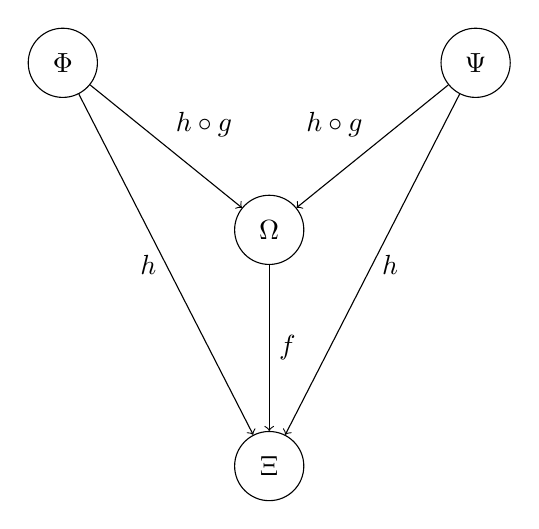
\begin{tikzpicture}[->,node distance=3cm]
\node[state] (Xi)                                        {$\Xi$}   ;
\node[state] (Omega) [above of=Xi]                       {$\Omega$};
\node[state] (Phi)   [above left of=Omega,  xshift=-5mm] {$\Phi$}  ;
\node[state] (Psi)   [above right of=Omega, xshift=5mm]  {$\Psi$}  ;
\path (Phi)   edge node [left]        {$h$}         (Xi)
              edge node [above right] {$h \circ g$} (Omega)
      (Psi)   edge node [right]       {$h$}         (Xi)
              edge node [above left]  {$h \circ g$} (Omega)
      (Omega) edge node [right]       {$f$}         (Xi);
\end{tikzpicture}
\end{center}

\begin{defin}
A formula $\Delta$ is a \textbf{canonical intersection} of two formulae $\Phi$ and $\Psi$, if and only if 
$\Delta$ is equivalent to $\Phi\cap\Psi$ and every function that assigns $\Phi$ and $\Psi$ to the same formula also assigns $\Delta$ to that formula.
We will introduce the following notation to express this:
\begin{align*}
\dfrac{\Phi \cap \Psi}{\Delta} \iff (\Phi\cap\Psi\equiv\Delta\land(\forall h : (\Phi\lhd h =\Psi\lhd h) \implies \Delta\lhd h=\Phi\lhd h))
\end{align*}
\end{defin}

\begin{lem}
If $\Delta$ is the canonical intersection of $\Phi$ and $\Psi$ then every free variable that appears in $\Delta$ must also appear in $\Phi$ and $\Psi$.
\begin{align*}
\dfrac{\Phi\cap\Psi}{\Delta}\implies\Delta^\mathcal{V}\subseteq\Phi^\mathcal{V}\cup\Psi^\mathcal{V}
\end{align*}
\end{lem}
\begin{proof}
Let us assume the negation.
Namely that there exists some free variable in $\Delta$ that is not in $\Phi$ or $\Psi$
\begin{align*}
\exists x : x \in \Delta^\mathcal{V} \land \neg (x \in \Phi^\mathcal{V}) \land \neg (x \in \Psi^\mathcal{V})
\end{align*}
Let us consider some function $h$ such that $\Phi\lhd h=\Psi\lhd h$.
By the definition of canonical intersection we know that it must be the case that $\Delta\lhd f = \Phi\lhd f$.
Now it must be the case that $h$ maps $x$ to some value, so we will make a new function $h'$ such that
for all values other than $x$, $h'$ behaves the same way as $h$, but for $h'(x)$ it maps to anything other than $h(x)$.
It doesn't matter what as long as it is different from what $h$ maps $x$ to.
Now it is clear that because $h'$ is the same as $h$ on the domains of $\Phi$ and $\Psi$, that $\Phi\lhd h' = \Phi\lhd h = \Psi\lhd h = \Psi\lhd h'$.
From our definition we can conclude that $\Delta \lhd h' = \Delta \lhd h$, thus via our first lemma $h' \mid \Delta^\mathcal{V} = h \mid \Delta^\mathcal{V}$.
However we already know this is false because we asserted that $h'(x) \neq h(x)$.
From this contradiction we can conclude that no such $x$ can exist.
\end{proof}
\begin{defin}
\textbf{The arrow number} of a formula $\Phi$, denoted $\Phi^\rightarrow$, will be defined as follows:
\begin{align*}
(\Phi_1\rightarrow\Phi_2)^\rightarrow &= 1 + \Phi_1^\rightarrow + \Phi_2^\rightarrow \\
(\neg\Phi_0)^\rightarrow &= \Phi_0^\rightarrow \\
\Phi \in \mathcal{V} \implies \Phi^\rightarrow &= 0\\
\Phi \in \mathcal{A} \implies \Phi^\rightarrow &= 0
\end{align*}
\end{defin}
This can also be thought of as the number of arrows appearing in the string that represents our formula.

\begin{thm}
Either the intersection of two formula is empty or there is a canonical intersection.
\begin{align*}
\forall \Phi,\Psi \in \mathcal{F} : \left(\Phi \cap \Psi = \left\{\right\} \lor \exists \Omega : \dfrac{\Phi \cap \Psi}{\Omega} \right)
\end{align*}
\end{thm}
\begin{proof}
This proof will be performed via structural induction.
To start we verify that this is in fact the case for atoms.
$\Phi \cap \Psi$ is the empty set if the atoms are different and is $\Phi$ if the atoms are the same.
This is pretty clear because no assignment can change a formula consisting only of an atom.
If $\Phi$ is the intersection it must be canonical because all assignments of $\Phi$ are also $\Phi$.

We can also see that for two free variables there is always a canonical intersection.
All the functions that assign two free variables to the same well formed formula are functions such that $f(\Phi) = f(\Psi)$ thus if we choose
our canonical intersection to be either $\Phi$ or $\Psi$ we will that this is indeed a intersection and it must be canonical.

Let us now consider that one of our formula is a free variable but the other is not.
Let us call the free variable $\phi$ and the other formula $\Psi$.
If $\phi$ appears in $\Psi$ then their intersection must be empty.
\begin{equation*}
\phi\in\Psi^\mathcal{V}\implies\phi\cap\Psi=\{\}
\end{equation*}
Otherwise it is clear that $\Psi$ is the canonical intersection.

Next we can see that if $\Phi$ and $\Psi$ have a canonical intersection $\Omega$ then $\neg\Omega$ is the canonical intersection of $\neg\Phi$ and $\Phi$.
This is clear by the fact that our definition of assignment carries through negation.
Equivalently if the intersection is empty the intersection of the negations must also be empty.

We now have an inductive proof that our proposition holds for all statements with arrow number $0$.

Now we will consider statements that do not have arrow number $0$.
We have already shown that statements with a negation at the top level are equivalent to a formula or empty set if removing the negation leaves us with formulae that have such an intersection, so we may go ahead and just consider statements that have an implication at the top level.
We consider
\begin{align*}
(\Phi_1 \rightarrow \Phi_2) \cap (\Psi_1 \rightarrow \Psi_2)
\end{align*}
Now if either $\Phi_1 \cap \Psi_1 = \{\}$ or $\Phi_2 \cap \Psi_2 = \{\}$ it is clear that the composite statement must be empty.
So we will only consider the case where $\exists \Lambda_1 : \dfrac{\Phi_1 \cap \Psi_1}{\Lambda_1}$ and $\exists \Lambda_2 : \dfrac{\Phi_2 \cap \Psi_2}{\Lambda_2}$.

Since $\Phi_1\cap \Psi_1 \equiv \Lambda_1$ we know, by lemma 4, that there is an assignment function $f$ that assigns both $\Phi_1$ and $\Psi_1$ to $\Lambda_1$.
Let us consider an arbitrary member of the intersection of $(\Phi_1\rightarrow\Phi_2)$ and $(\Psi_1\rightarrow\Psi_2)$, let us call it $(\Xi_1\rightarrow\Xi_2)$.
If we call the function that assigns both $(\Phi_1\rightarrow\Phi_2)$ and $(\Psi_1\rightarrow\Psi_2)$ to $(\Xi_1\rightarrow\Xi_2)$, $h$.
$h$ must assign $\Phi_1$ and $\Psi_1$ to the same well formed formula (namely $\Xi_1$),
thus by the definitions of equivalent formulae it must be the case that there is a function $g$ that assigns $\Lambda_1$ to $\Phi_1\lhd h$ and $\Psi_1\lhd h$.
Thus
\begin{align*}
\Phi \lhd (f\diamond g) = \Phi_1 \lhd h \\
\Psi \lhd (f\diamond g) = \Psi_1 \lhd h
\end{align*}
From Lemma 1 we then show that
\begin{align*}
(f\diamond g) \mid \Phi_1^\mathcal{V} \cup \Psi_1^\mathcal{V} = h \mid \Phi_1^\mathcal{V} \cup \Psi_1^\mathcal{V} 
\end{align*}
Now it is trivially true that if $\mathrm{id}$ is the function that maps every free variable to itself.
\begin{align*}
(\mathrm{id}\diamond h) = h
\end{align*}
So if we define two new functions $f'$ and $g'$ such that
\begin{align*}
f' (x) = \begin{cases}
f (x) & x \in \Phi_1^\mathcal{V} \cup \Psi_1^\mathcal{V} \\ 
x & \mathrm{otherwise}
\end{cases}\\
g'(x) = \begin{cases}
g (x) & x \in \Phi_1^\mathcal{V} \cup \Psi_1^\mathcal{V} \\ 
h (x) & \mathrm{otherwise}
\end{cases}
\end{align*}
It then must be the case that
\begin{align*}
(f'\diamond g') = h
\end{align*}
This means that for any formula $\Xi$ in the intersection, that
\begin{align*}
((\Phi_1\rightarrow\Phi_2)\lhd f')\lhd g' = \Xi \\
((\Psi_1\rightarrow\Psi_2)\lhd f')\lhd g' = \Xi
\end{align*}
And since $f'$ is not dependent on $\Xi$ we can say that
\begin{align*}
(\Phi_1\rightarrow\Phi_2)\cap(\Psi_1\rightarrow\Psi_2)
&= ((\Phi_1\rightarrow\Phi_2)\lhd f')\cap((\Psi_1\rightarrow\Psi_2)\lhd f') \\
&= (\Lambda_1\rightarrow(\Phi_2\lhd f'))\cap(\Lambda_1\rightarrow(\Psi_2\lhd f'))
\end{align*}
Since $\Lambda_1$ is already equal to itself, any assignment of $\Lambda_1$ will be equal to itself.
Thus an assignment will assign both $(\Phi_2\lhd f')$ and $(\Psi_2\lhd f')$ to the same formula if and only if it assigns both $(\Lambda_1\rightarrow(\Phi_2\lhd f'))$ and $(\Lambda_1\rightarrow(\Psi_2\lhd f'))$ to the same formula.
\begin{equation*}
(\Phi_2\lhd f')\lhd k =(\Psi_2\lhd f')\lhd k \iff
(\Lambda_1\rightarrow(\Phi_2\lhd f')) \lhd k = (\Lambda_1\rightarrow(\Psi_2\lhd f')) \lhd k
\end{equation*}
From this fact it is clear that $(\Phi_2\lhd f')\cap(\Psi_2\lhd f')$ is empty if and only if $(\Lambda_1\rightarrow(\Phi_2\lhd f'))\cap(\Lambda_1\rightarrow(\Psi_2\lhd f'))$ is also empty.
If $(\Phi_2\lhd f')\cap(\Psi_2\lhd f')$ is non-empty we see that
\begin{align*}
\forall k :
(\Phi_2\lhd f') \lhd k = (\Psi_2\lhd f') \lhd k
&\iff ((\Lambda_1\lhd k)\rightarrow ((\Phi_2\lhd f')\lhd k)) = ((\Lambda_1\lhd k)\rightarrow ((\Psi_2\lhd f')\lhd k)) \\
&\iff (\Lambda_1\rightarrow (\Phi_2\lhd f'))\lhd k = (\Lambda_1\rightarrow (\Psi_2\lhd f'))\lhd k
\end{align*}
Thus from here if $(\Phi_2\lhd f')\cap(\Psi_2\lhd f') \equiv \Omega$ then by lemma 4 there must be an assignment $k$ from both $(\Phi_2\lhd f')$ and $(\Psi_2\lhd f')$ to $\Omega$, 
which entails that every assignment into the intersection must be of the form $(k \diamond l)$.
From the above result this means that every assignment from $(\Lambda_1\rightarrow (\Phi_2\lhd f'))$ and $(\Lambda_1\rightarrow (\Psi_2\lhd f'))$ into their intersection must also be of the form $(k \diamond l)$.
If we take $(\Lambda_1\rightarrow (\Psi_2\lhd f'))\lhd k$, it must be a formula and it must be equivalent to the intersection.
Thus if there is some formula that is equivalent to $(\Phi_2\lhd f')\cap(\Psi_2\lhd f')$ there must also be an formula that is equivalent to $(\Phi_1 \rightarrow \Phi_2) \cap (\Psi_1\rightarrow \Psi_2)$.

Now we will take a moment to prove that $(\Phi_2\lhd f')^\mathcal{V}\cup(\Psi_2\lhd f')^\mathcal{V} \subseteq (\Phi_1\rightarrow\Phi_2)^\mathcal{V} \cup (\Psi_1\rightarrow\Psi_2)^\mathcal{V}$.
\begin{subproof}
We can use lemma 2 to show
\begin{align*}
(\Phi_2\lhd f')^\mathcal{V}\cup(\Psi_2\lhd f')^\mathcal{V}
= \bigcup_{\delta \in \Phi_2^\mathcal{V}\cup\Psi_2^\mathcal{V}}(f'(\delta))^\mathcal{V}
\end{align*}
Since $\Lambda_1$ is a canonical intersection we know that $\Lambda_1^\mathcal{V} \subseteq \Phi_1^\mathcal{V}\cup\Psi_1^\mathcal{V}$, thus $f'$ must map every variable in $\Phi_1^\mathcal{V}\cup\Psi_1^\mathcal{V}$ to another variable in $\Phi_1^\mathcal{V}\cup\Psi_1^\mathcal{V}$, and since $f'$ is the id everywhere else we know that
\begin{align*}
(\Phi_2\lhd f')^\mathcal{V}\cup(\Psi_2\lhd f')^\mathcal{V}
= \bigcup_{\delta \in \Phi_2^\mathcal{V}\cup\Psi_2^\mathcal{V}}(f'(\delta))^\mathcal{V}
\subseteq \Phi_1^\mathcal{V}\cup\Phi_2^\mathcal{V} \cup \Psi_1^\mathcal{V}\cup\Psi_2^\mathcal{V}
\end{align*}
And by definition we can also say that:
\begin{align*}
(\Phi_1\rightarrow\Phi_2)^\mathcal{V} \cup (\Psi_1\rightarrow\Psi_2)^\mathcal{V}
= \Phi_1^\mathcal{V}\cup\Phi_2^\mathcal{V} \cup \Psi_1^\mathcal{V}\cup\Psi_2^\mathcal{V}
\end{align*}
Thus
\begin{align*}
(\Phi_2\lhd f')^\mathcal{V}\cup(\Psi_2\lhd f')^\mathcal{V} \subseteq (\Phi_1\rightarrow\Phi_2)^\mathcal{V} \cup (\Psi_1\rightarrow\Psi_2)^\mathcal{V}
\end{align*}
\end{subproof}

Now we wish to show that if the arrow number of $\Phi_2\lhd f'$ is greater than or equal to the arrow number of $\Phi$ then $(\Phi_2\lhd f')^\mathcal{V}\subset\Phi^\mathcal{V}$.
\begin{subproof}
We know that $\Phi_2$ must have a lower arrow number than $\Phi$ because $\Phi$ by definition has an arrow number equal to the sum of the arrow numbers of $\Phi_1$, $\Phi_2$ and $1$.
Thus in order for the arrow number to be greater or equal to that of $\Phi$, some free variable must assign itself to some formula with a nonzero arrow number.
Since this free variable, which we will call $\phi$, is not assigned to itself we know that it must be present in $\Phi_1^\mathcal{V}$ or $\Psi_1^\mathcal{V}$.
Now in order for the free variable $\phi$ to be present in $\Phi_2\lhd f'$, we must have some cycle such that
\begin{gather*}
\phi_1 \in f'(\phi)\\
\phi_2 \in f'(\phi_1)\\
\phi_3 \in f'(\phi_2)\\
 \vdots \\
\phi_n \in f'(\phi_{n-1})\\
\phi \in f'(\phi_n)
\end{gather*} 
However since for all $n$, $\phi_n$ appears in $\Phi_1$ or $\Psi_1$, and $f'$ assigns those two to their canonical intersection, it is clear that such a chain cannot exist,
thus $\phi$ cannot appear in $\Phi_2\lhd f'$, forcing $(\Phi_2\lhd f')^\mathcal{V}$ to be a strict subset of $\Phi^\mathcal{V}$.
\end{subproof}

Since the arrow number of our statement can only be larger if the number of free variables is smaller and the the number of free variables can never increase,
we can show by induction (with the already established base case of arrow number of $0$) our proposition holds for formulae of any arrow number.

\end{proof}

As with many inductive theorems we can use this to very easily create a recursive algorithm to find a canonical intersection if such a thing exists.
In order to do this one defines a function that finds an assignment to a canonical intersection following the construction steps outlined in the proof.
We will not go into the algorithm in detail, since it would mostly just be a repeat of the proof above, however we do have an implementation of it in the file
\texttt{intersection.hs}.

This particular tool is very powerful because we can rephrase a bunch of problems we will encounter as finding an intersection between two formulae.

\subsection{Hilbert Systems}

A Hilbert Axiom system is a deductive system with is equipped with a two inference rules, axiom introduction and modus ponens.
A Hilbert system has a set of Axioms, which are what differentiate different Hilbert systems
A proof in a Hilbert system is structured as a sequence of well-formed statements, $S$, each justified by the application of a inference rule.
A statement $\Phi$ can be justified by modus ponens iff there is an assignment $f$ such that $\phi\lhd f$ and $(\phi\rightarrow\psi)\lhd f$ appear earlier in the sequence and
$\phi\lhd f=\Phi$.
A statement can be justified via axiom instantiation iff it is an assignment of one of our axioms.

\subsection{\L ukasiewicz Axiom system}
The \L ukasiewicz Axiom system is a Hilbert system with the following axioms:
\begin{gather*}
\phi \rightarrow (\psi \rightarrow \phi) \\
(\phi\rightarrow(\psi\rightarrow\chi))\rightarrow((\phi\rightarrow\psi)\rightarrow(\phi\rightarrow\chi)) \\
(\neg\phi\rightarrow\neg\psi)\rightarrow(\psi\rightarrow\phi)
\end{gather*}

\section{Proof Golf}

Now that we have built a number of really powerful tools and definitions we can begin to consider actually proving things.
The first toy problem we will work with is a proof of $(A\rightarrow A)$ in the \L ukasiewicz system.
This is a good problem because it is not that difficult to find a somewhat short proof of this statement.
In fact with a little effort one would probably find the following 5 step proof.
\begin{gather*}
(A\rightarrow(A\rightarrow A)) \tag*{L.S.1}\\
(A\rightarrow((A\rightarrow A)\rightarrow A)) \tag*{L.S.1}\\
((A\rightarrow((A\rightarrow A)\rightarrow A))\rightarrow((A\rightarrow(A\rightarrow A))\rightarrow(A\rightarrow A)) \tag*{L.S.2}\\
((A\rightarrow(A\rightarrow A))\rightarrow(A\rightarrow A)) \tag*{M.P. (2,3)}\\
(A\rightarrow A) \tag*{M.P. (1,4)}
\end{gather*}
Now that we have the proof we want to know if there is a shorter proof we can come up with, that is golf our proof.
It turns out that there is not a shorter proof, but in order to know this we will have to prove it.
The issue that one first meets in proving that there is no proof of a certain size is the fact that the search space is infinite.
There are an infinite number of ways to instantiate each axiom, so we cannot check each one individually.
In order to get around this we use a fairly simple method, instead of talking about specific well formed formulae, we use formulae with free variables to talk more generally about
the infinite possibilities.
This borrows a bit from the principle of lazy evaluation.
We allow values to be unknown until we are forced to evaluate them.

\begin{thm}
There is no proof of $A \rightarrow A$ in the \L ukasiewicz system that is less than 5 steps long.
\end{thm}
\begin{proof}
In order to prove that no such proof exists we will attempt to construct such a proof.
We will despite our best efforts fail to do so demonstrating the impossibility of the task.

We will start our proof at the end.
We know that the statement $(A \rightarrow A)$ must appear in the proof,
and that any steps after it are extraneous and can be removed.
Thus $(A \rightarrow A)$ must be the last step of the proof.
We will label this step $\alpha$

\begin{align*}
(A \rightarrow A) \tag*{($\alpha$)}\\
\end{align*}

By the above algorithm we know that $(A \rightarrow A)$ does not fit the form of any of our axioms.
This means that we must have arrived at it from modus ponens.

\begin{align*}
(A \rightarrow A) \tag*{Modus Ponens ($\alpha$)}\\
\end{align*}

Since we arrived at this from modus ponens we know that there must be earlier statements of the form $\phi$ and $(\phi \rightarrow (A \rightarrow A))$.
Since all statements are finite we also know that there is no $\phi$ such that

\begin{align*}
\phi = \phi \rightarrow (A \rightarrow A)
\end{align*}

Thus the two statements must be separate.

\begin{gather*}
\phi \tag{$\gamma$}\\
(\phi \rightarrow (A \rightarrow A)) \tag{$\beta$}\\
(A \rightarrow) A \tag*{Modus Ponens ($\gamma$,$\beta$) ($\alpha$)}\\
\end{gather*}

Using our algorithm for intersection we find that we can express $(\phi \rightarrow (A \rightarrow A))$ as a statement of L.S.1 if $\phi = A$,
however doing so would mean that our proof would need to include a proof of $A$.
Since $A$ clearly is independent of our axioms we know that the statement cannot be a reference to L.S.1.

Via our algorithm we know that $(\phi \rightarrow (A \rightarrow A))$ has an empty intersection with L.S.2 and thus cannot be justified with L.S.2.

Lastly if we set $\phi$ equal to $(\neg A \rightarrow \neg A)$ we will find that L.S.3 allows us to conclude our statement.

\begin{gather*}
(\neg A \rightarrow \neg A) \tag{$\gamma$}\\
((\neg A \rightarrow \neg A) \rightarrow (A \rightarrow A)) \tag*{L.S.3 ($\beta$)} \\
(A \rightarrow A) \tag*{Modus Ponens ($\gamma$,$\beta$) ($\alpha$)}\\
\end{gather*}

Now our intersection algorithm tells us that $(\neg A \rightarrow \neg A)$ must be derived via modus ponens.
This gives us a proof of the form:

\begin{gather*}
\psi \tag{$\epsilon$}\\
(\psi \rightarrow (\neg A \rightarrow \neg A)) \tag{$\delta$} \\
\phantom{\text{Modus Ponens ($\epsilon$, $\delta$) ($\gamma$)}} (\neg A \rightarrow \neg A) \tag*{Modus Ponens ($\epsilon$, $\delta$) ($\gamma$)}\\
((\neg A \rightarrow \neg A) \rightarrow (A \rightarrow A)) \tag*{L.S.3 ($\beta$)} \\
(A \rightarrow A) \tag*{Modus Ponens ($\gamma$,$\beta$) ($\alpha$)}\\
\end{gather*}

Now since we are looking for a proof with 4 steps we know that it must be the case that $\psi$ is equal to $(\neg A \rightarrow \neg A) \rightarrow (A \rightarrow A)$, otherwise we would have 5 steps.

\begin{gather*}
(\psi \rightarrow (\neg A \rightarrow \neg A)) \tag{$\delta$} \\
((\neg A \rightarrow \neg A) \rightarrow (A \rightarrow A)) \tag*{L.S.3 ($\beta$)} \\
\phantom{\text{Modus Ponens ($\beta$, $\delta$) ($\gamma$)}} (\neg A \rightarrow \neg A) \tag*{Modus Ponens ($\beta$, $\delta$) ($\gamma$)}\\
(A \rightarrow A) \tag*{Modus Ponens ($\gamma$,$\beta$) ($\alpha$)}
\end{gather*}

Checking with our algorithm we find that there is no way to instantiate our first statement as one of the axioms.
Thus it must be modus ponens that introduces it, however it cannot be arrived at via modus ponens from any of the existing formula, meaning we need new steps if we are to continue.

Now we backtrace to the last decision we made.
We chose to represent $(\phi \rightarrow (A \rightarrow A))$ as L.S.3.
Since that arrived us at an incorrect conclusion we know that it cannot be the case that in a four step proof that step is introduced by L.S.3.
Since we have removed all of the axioms as possibilities to introduce $(\phi \rightarrow (A \rightarrow A))$ we know that it is introduced by modus ponens.

\begin{gather*}
\phi \tag{$\gamma$}\\
\psi \tag{$\epsilon$}\\
\psi \rightarrow (\phi \rightarrow (A \rightarrow A)) \tag{$\delta$}\\
\phantom{\text{Modus Ponens ($\epsilon$, $\delta$) ($\beta$)}} \phi \rightarrow (A \rightarrow A) \tag*{Modus Ponens ($\epsilon$, $\delta$) ($\beta$)} \\
\phantom{\text{Modus Ponens ($\gamma$, $\beta$) ($\alpha$)}} (A \rightarrow A) \tag*{Modus Ponens ($\gamma$, $\beta$) ($\alpha$)}
\end{gather*}

Since we have 5 claims here we know that in order to reduce our proof to 4 steps we must have two of them that are equal.
It is clear that no statement containing $\phi$ can be equal to $\phi$ and the same goes for $\psi$.
We also know that if a statement $\chi$ that relies on a statement $\omega$, it must be the case that $\chi \neq \omega$ otherwise our proof would be circular.

Of the remaining formulae that could be equal there is only one pair that has the same form.
This leaves us to say that $\phi = \psi$. 

\begin{gather*}
\phi \tag{$\gamma$}\\
\phi \rightarrow (\phi \rightarrow (A \rightarrow A)) \tag{$\delta$}\\
\phantom{\text{Modus Ponens ($\gamma$, $\delta$) ($\beta$)}} \phi \rightarrow (A \rightarrow A) \tag*{Modus Ponens ($\gamma$, $\delta$) ($\beta$)} \\
\phantom{\text{Modus Ponens ($\gamma$, $\beta$) ($\alpha$)}} (A \rightarrow A) \tag*{Modus Ponens ($\gamma$, $\beta$) ($\alpha$)}
\end{gather*}

Our remaining statements must be instantiations of our axioms because any use of modus ponens would add new steps to the proof.
If we start with the sentence $\phi \rightarrow (\phi \rightarrow (A \rightarrow A))$ we will find it can only be instantiated by L.S.1.

\begin{gather*}
(A\rightarrow A) \tag{$\gamma$}\\
(A\rightarrow A) \rightarrow ((A\rightarrow A) \rightarrow (A \rightarrow A)) \tag*{L.S.1 ($\delta$)}\\
\phantom{\text{Modus Ponens ($\gamma$, $\delta$) ($\beta$)}} (A\rightarrow A) \rightarrow (A \rightarrow A) \tag*{Modus Ponens ($\gamma$, $\delta$) ($\beta$)} \\
\phantom{\text{Modus Ponens ($\gamma$, $\beta$) ($\alpha$)}} (A \rightarrow A) \tag*{Modus Ponens ($\gamma$, $\beta$) ($\alpha$)}
\end{gather*}

Now in order to make this proof valid we must proof $A \rightarrow A$ in 1 step.
This would require the instantiation of an axiom and we already know that this is impossible.

Thus there is no proof of $A \rightarrow A$ that is 4 steps or shorter.
\end{proof}

\section{Algorithmically Finding Optimal Proofs}

This proof that we have constructed actually can be extended into a general approach for proving a proof is minimal, which can be codified directly into an algorithm.

Will will first create a \textbf{partial proof} type.
A partial proof consists of two sets of formulae.
One set for formulae that have been justified and one for those lacking justifications.
A partial proof represents, as its name would suggest, a proof that has not yet been completed.
A partial proof is complete once every formula has a justification.

Our algorithm will mostly operate on a priority queue of these partial proofs.
Our priority function will be such that partial proofs with less overall formulae (number of justified and unjustified formulae) will always have higher priority.
In the case of a tie on that metric partial proofs with less unjustified formulae will take priority.

At each step of our algorithm we will pop a single partial proof out of the priority queue to examine it.
We will attempt to justify a single formula from our set of unjustified formulae.
In practice it doesn't matter which one we choose but in our actual implementation we implement our unjustified formula as a queue, so which formula is selected is deterministic.

In order to find all the ways to justify a single formula, we will first compare our formula to all of our axioms using our intersection algorithm.
If the intersection is empty no instance of it is an instance of our algorithm, however if there is a canonical intersection that represents the most general formula
which is an instance of both the original formula and the axiom.
So if there is an intersection we can justify our by applying the assignment found by our algorithm to every formula in our partial proof, and moving the relevant formula to the justified proof set.

Once we have found all the ways we can justify a statement with axioms we must find all the ways in which it can be justified via modus ponens.
At first it might seem like there is only 1 way this can be done.
To justify the formula $\Phi$ we must add the formulae $\psi$ and $(\psi \rightarrow \Phi)$, to our unjustified formulae. 
However this doesn't account for formula in which a single statement is use in two separate modus ponens.
For example consider the following proof mock up.
Here modus ponens is represented by arrows, pointing from the formulae it operates to the formula it justifies.

\begin{center}
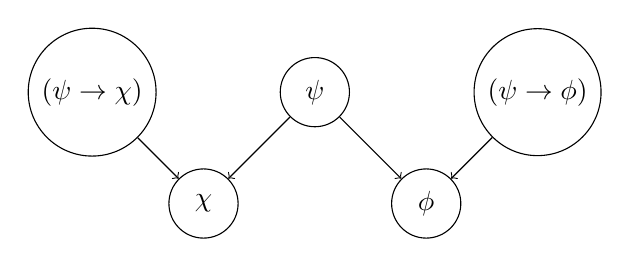
\begin{tikzpicture}[->,node distance=2cm]
\node[state] (psi) {$\psi$} ;
\node[state] (phi) [below right of=psi] {$\phi$} ;
\node[state] (chi) [below left  of=psi] {$\chi$} ;
\node[state] (psiimphi) [above right of=phi] {$(\psi\rightarrow\phi)$} ;
\node[state] (psiimchi) [above left  of=chi] {$(\psi\rightarrow\chi)$} ;

\path (psi)      edge (phi) 
                 edge (chi)
      (psiimphi) edge (phi)
      (psiimchi) edge (chi);
    
\end{tikzpicture}
\end{center}

Clearly this proof structure cannot be achieved via our naive method of performing modus ponens.
In order to create proofs with this type of structure we need combine the new statements that we are adding with existing statements.
We can do this with our intersection algorithm.
So in order to capture all the way modus ponens can justify a formula we need to create the formulae $\psi$ and $(\psi\rightarrow\Phi)$ and then unify these formulae every way we possibly can with existing formulae.

However this opens us up to the possibility of circular proofs.
So we need to add the additional constraint that we don't unify any statement with a statement that relies on it.
This will mean we will need to keep track of what statements rely on each other as we run through the proof.

Once we have all the ways to justify a single formula we will put all these new partial proofs back in the priority queue and we can repeat the process.

Once we have a proof with no unjustified formulae we stop because we have found the shortest possible proof.

\subsection{Optimizations}

A couple of optimizations can be made to this approach.
The first is rather simple, every time we attempt to justify a formula we compare it to all other existing formulae, justified or not.
If it is equal to another formula in our proof our proof can never be the shortest.
If the one of the copies relies on the other for justification (via modus ponens) then whatever route taken to prove a statement from itself must be extraneous.
If the copies are not reliant on each other then they could be rewritten as a single formula, and in fact there must be another partial proof that has done just that.
So if we discover two equal formula we simply remove the partial proof from our queue without any replacement.
This optimization has been implemented in the included code.

Another optimization we can make that applies only two consistent axiom systems, is to throw out partial proofs that require unprovable formulae to be proven.
For example in our proof that $(A\rightarrow A)$ requires 5 steps to prove we throw out a partial proof that requires us to prove $A$.
We do have to note that determining if a formula is provable is equivalent to SAT solving and thus there is no know polynomial time algorithm to do so in general.
It is thus better to use a heuristic check instead, say throwing out all partial proof that require us to prove an atom.
This optimization has not been implemented in our included code because our code is intended to be useable for inconsistent axiom systems.

\section{Our Implementation}

For demonstration purposes we have written an implementation of the described algorithms in Haskell.

\subsection{Usage}

The code can be tested by creating a new Haskell file and importing the libraries \texttt{Prover} and \texttt{Formula}.
You can create a new formula using the constructors from the \texttt{Formula} module.
The constructors are, \texttt{If} which takes 2 formulae in prefix notation which represents our $\rightarrow$,
\texttt{Neg} which takes a single formula as a prefix and represents the negation of that formula,
\texttt{Atom} which takes a \texttt{Char} and creates the atom which is identified by that character (for example $A$ is \texttt{Atom 'A'}),
\texttt{Variable} which takes an \texttt{Int} and creates a free variable which is identified by that integer.

For example if we wanted to construct the formula $(A\rightarrow A)$ we might write

\begin{equation*}
\texttt{myFormula = If (Atom 'A') (Atom 'A')}
\end{equation*}

Now to get an axiom system we can either create our own as detailed in the next section or we can import one of the two pre-made systems.
The modules \texttt{Lukasiewicz} and \texttt{Meredith} each contain an axiom system contained in the variable \texttt{axioms}.

If we wish to then find the shortest proof of a formula we can then call it with
\begin{align*}
&\texttt{main :: IO ()} \\
&\texttt{main = print \$ findProof myAxioms \$ format [myFormula]}
\end{align*}

\subsection{Output}

If compiled and run the output should be placed in the console however it takes a bit of knowledge to actually read the output.
As an example let us take a look at the output when we ask it to prove $(A\rightarrow A)$
\begin{align*}
&\texttt{Just} \\
&\texttt{(Axiom 1) (A -> (\{9\} -> A))} \\
&\texttt{(Axiom 1) (A -> ((\{9\} -> A) -> A))} \\
&\texttt{(Axiom 2) ((A -> ((\{9\} -> A) -> A)) -> ((A -> (\{9\} -> A)) -> (A -> A)))} \\
&\texttt{(Modus Ponens) ((A -> (\{9\} -> A)) -> (A -> A))} \\
&\texttt{(Modus Ponens) (A -> A)} \\
\end{align*}
The first line \texttt{Just} is not very important, it will always be output mostly for internal reasons.
It can be trimmed if desired but we decided not to.
Other than that each line is a line of the proof with its justification on the left and its formula on the right.
A number enclosed in brackets is a free variable.
Two with the same number are the same free variable but other than that the actual number doesn't mean anything specific.
Now technically a free variable should never appear in a proper proof, but here the solver is telling you that you can put anything in for \texttt{\{9\}} as long as you put the same thing in everywhere.

\subsection{Axiom Systems}

Besides the existing axiom systems in the modules \texttt{Meredith} and \texttt{Lukasiewicz}, additional axiom systems can be made.
An axiom system is simply a list of axioms which can be created in a two ways.
The first is to import the module \texttt{Axiom} and use the function \texttt{buildAxiom} to create an axiom from a formula with free variables.
For example here is how we would make the law of contraposition
\begin{align*}
\texttt{myAxiom = buildAxiom \$ If(If(Neg(Variable 0))(Neg(Variable 1)))(If(Variable 1)(Variable 0))}
\end{align*}
The other is to use the raw axiom constructors also from the \texttt{Axiom} module, you can see an example of this by opening either of the pre-made modules.

\subsection{Unintended Features}
There are a number of unintended features that the implementation has.
The first is that you can ask the prover to prove statements that have free variables in them.
In these cases the prover will fill in the free variables as it wishes to make the proof as short as possible.
For example we can ask the prover to prove $(\phi\rightarrow\phi)$ and it will tell us
\begin{align*}
&\texttt{Just}\\
&\texttt{(Axiom 1) (\{4\} -> (\{5\} -> \{4\}))}\\
&\texttt{(Axiom 1) ((\{4\} -> (\{5\} -> \{4\})) -> ((\{4\} -> (\{5\} -> \{4\})) -> (\{4\} -> (\{5\} -> \{4\}))))}\\
&\texttt{(Modus Ponens) ((\{4\} -> (\{5\} -> \{4\})) -> (\{4\} -> (\{5\} -> \{4\})))}
\end{align*} 

We can also ask the prover to prove multiple statements in the same proof by including them both in the list of \texttt{format}. The prover will construct the shortest proof that includes both of those statements.

Lastly (this is unintended feature is less unintended because we made specific modifications to make it more usable) one can use assumptions in their proofs.
This is done by adding formulae to the already justified list of formulae.
These can be given any justification but we have a built in justification \texttt{Assume} just for this purpose.
In order to do this you have to abandon \texttt{format} and instead use \texttt{formatWithAssumptions} which takes two lists of formulae, the first assumptions and the second goals.

\subsection{Improvements and Shortcomings}

There are a number of improvements that could be made to the current implementation.
The first one would be to replace the rather slow implementation of a priority queue with a better data structure.
The current queue is quite naive and could greatly benefit from being reimplemented.

We would also like to label which formula modus ponens is being used upon in the output.
However for technical reasons this was very difficult and we decided that it would be more effort than it was worth to do so on our tight time budget.

Our implementation also lacks a few generalities that could be possible.
For example other operators other than implication could very easily be added, since the system cares very little about semantics.
It would be quite possible to allow users to define their own binary connectives for use in proofs.

Along the same thread it would definitely be possible to add user defined inference rules, in place of or along side modus ponens.
Our algorithm is general enough that the semantics of modus ponens are not important.
Such inference rules might include Nicod's modus ponens.

\end{document}
